\section{The U-Net}

The \emph{U-Net} is a network achitecture first proposed by \Citeauthor{ronnebergerUNetConvolutionalNetworks2015} in 2015 for application in biomedical segmentation tasks, for example segmenting cell borders in microscopic images of HeLa cells. 
The challenges the authors were facing at the time are similar to the ones in this thesis, where training data for biomedical segmentation tasks was scarce, which is why the U-Net was makes sense as a starting point for the problem of droplet segmentation.

It is a fully convolutional network, which were on the rise to surpass older state of the art neural networks for classification tasks at the time. 
The network employs an \emph{encoder-decoder} structure, meaning the architecture consists of a contracting path and a expanding path, the \emph{encoder} and \emph{decoder} respectively, as seen in Figure \ref{fig:unet}.

\begin{figure}[htbp]
    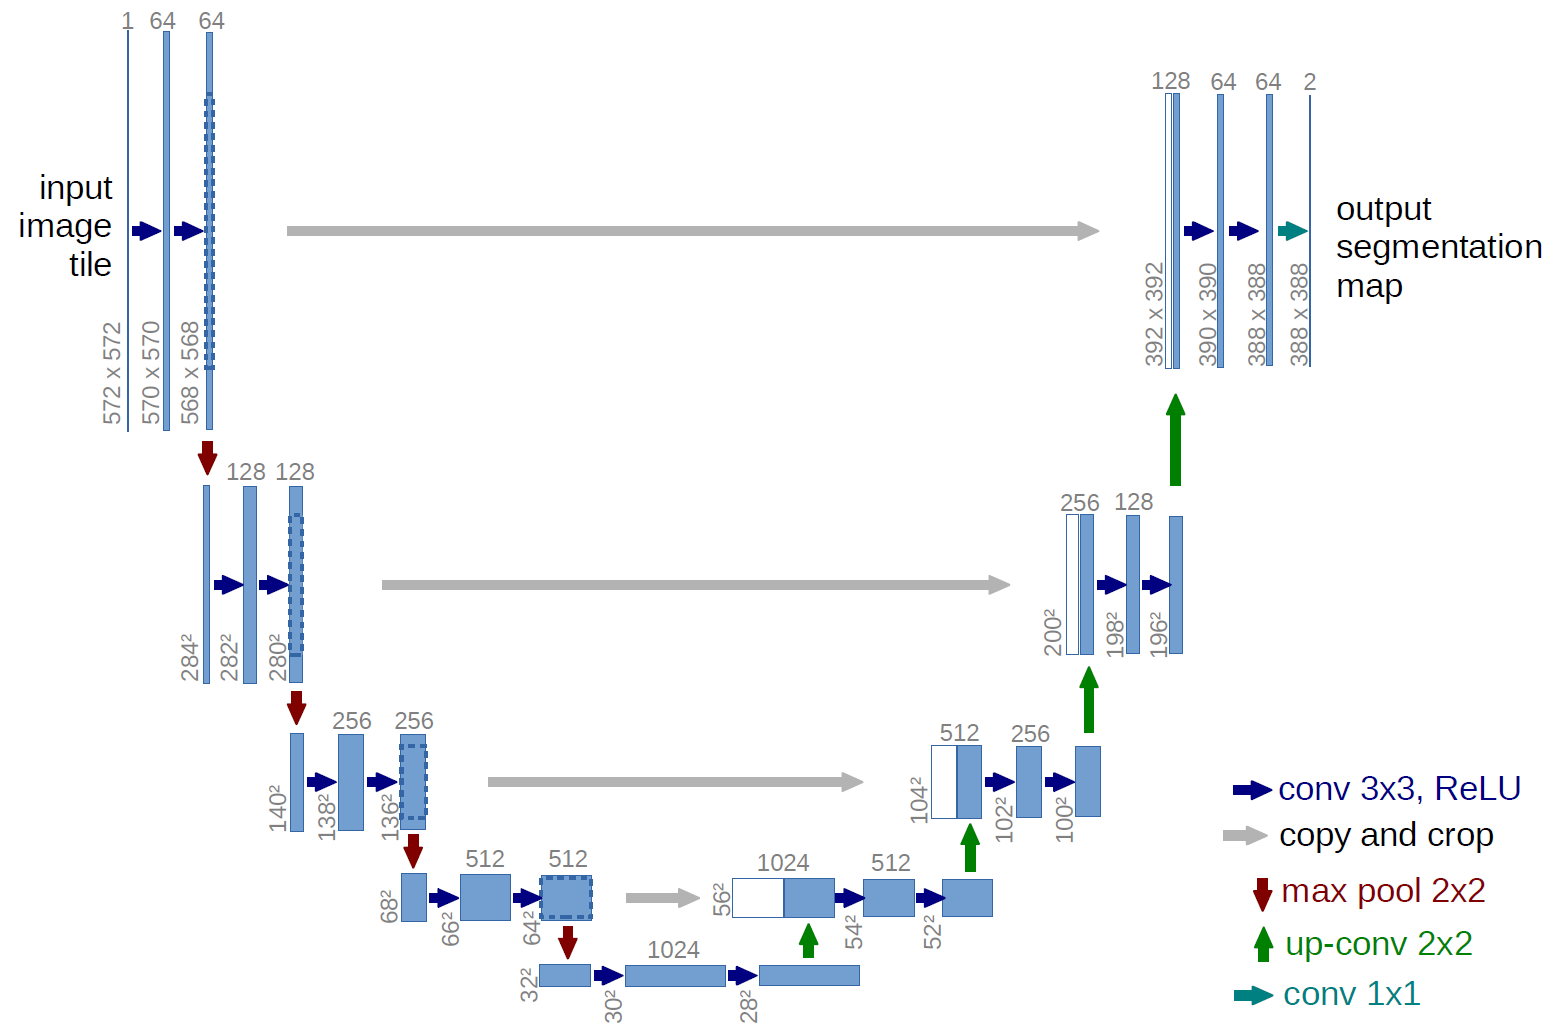
\includegraphics[width=\textwidth]{images/unet.png}
    \caption{The original U-Net architecture proposed in \cite{ronnebergerUNetConvolutionalNetworks2015}, for an example of a $572\times 572$ input, with the number of channels of the layer written above the blue boxes representing the feature map after each layer passthrough. The legend shows which operation was used between each feature map.}
    \label{fig:unet}
\end{figure}

The encoder path computes a number of features at four different spatial input sizes with two $3\times 3$ convolutions followed by a ReLu, which are then downsampled by a $2\times 2$ max-pooling layer. 
With each of these blocks, the spatial resolution is halfed along each axis, while the number of feature channels is doubled.

The features output by each block depend on different sized regions of the initial input. 

The values of blocks with high spatial resolution consider only small patches in the input image, while a lot of pixels influence each value for the lower blocks. 
The large \emph{perceptive field} of the lower blocks allow for rich contextual information to be encoded in their feature maps.

In a classification problem, such contracing networks would be used by feeding the highly dense information of the last encoder block to a few fully connected layers which make the final classification decision. 
In this case, since a classification for each pixel is needed, the encoded information must now be scaled back up to the desired resolution.

The decoder path is symmetrical to the encoder path, halving the number of feature channels in each block and upsampling the spatial resolution by using $2\times 2$ \emph{transposed convolutions}, which act like a backwards pass through a normal convolution.
After the last upsampling block a final $1\times 1$ convolution is used to decide the final class for each pixel.

However, as is, this structure has a key flaw when it comes to creating segmentation masks. While it is feasable to deduce general locations of objects from the highly contextual encoder features, it is difficult to infer their exact boundaries, because the spatial resolution has been compressed so much. 

This is where another key aspect of the U-Net architecture comes in. 
By concatenating the outputs of each encoder block to the input of their respective decoder block, we allow the decoder to not only utlize the context information provided by the last enocoder layers, but also the very localized features of the high resolution blocks.

This combination allows the U-Net to predict the correct classes along with their precise spatial location.

The U-Net outperformed its predecessors by a large margin and has since been developed further. Its concepts still serve as the basis for popular segmentation networks.\\

One way in which the original U-Net architecture is often modified, is using more sophisticated models for the encoder module, which is the approach taken in this thesis. 
Obtaining better features has proven itself to lead to better overall results, so investing more capability in the encoder structure is often a good idea. 

This also comes with the added benefit that pretrained weights for common feature extractors like the \emph{ResNet} (more in \ref{sec:resnet}) are readily available. 